% Auto-generated HRS Manuscript Figure & Table Includes

\begin{figure*}[t]
    \centering
    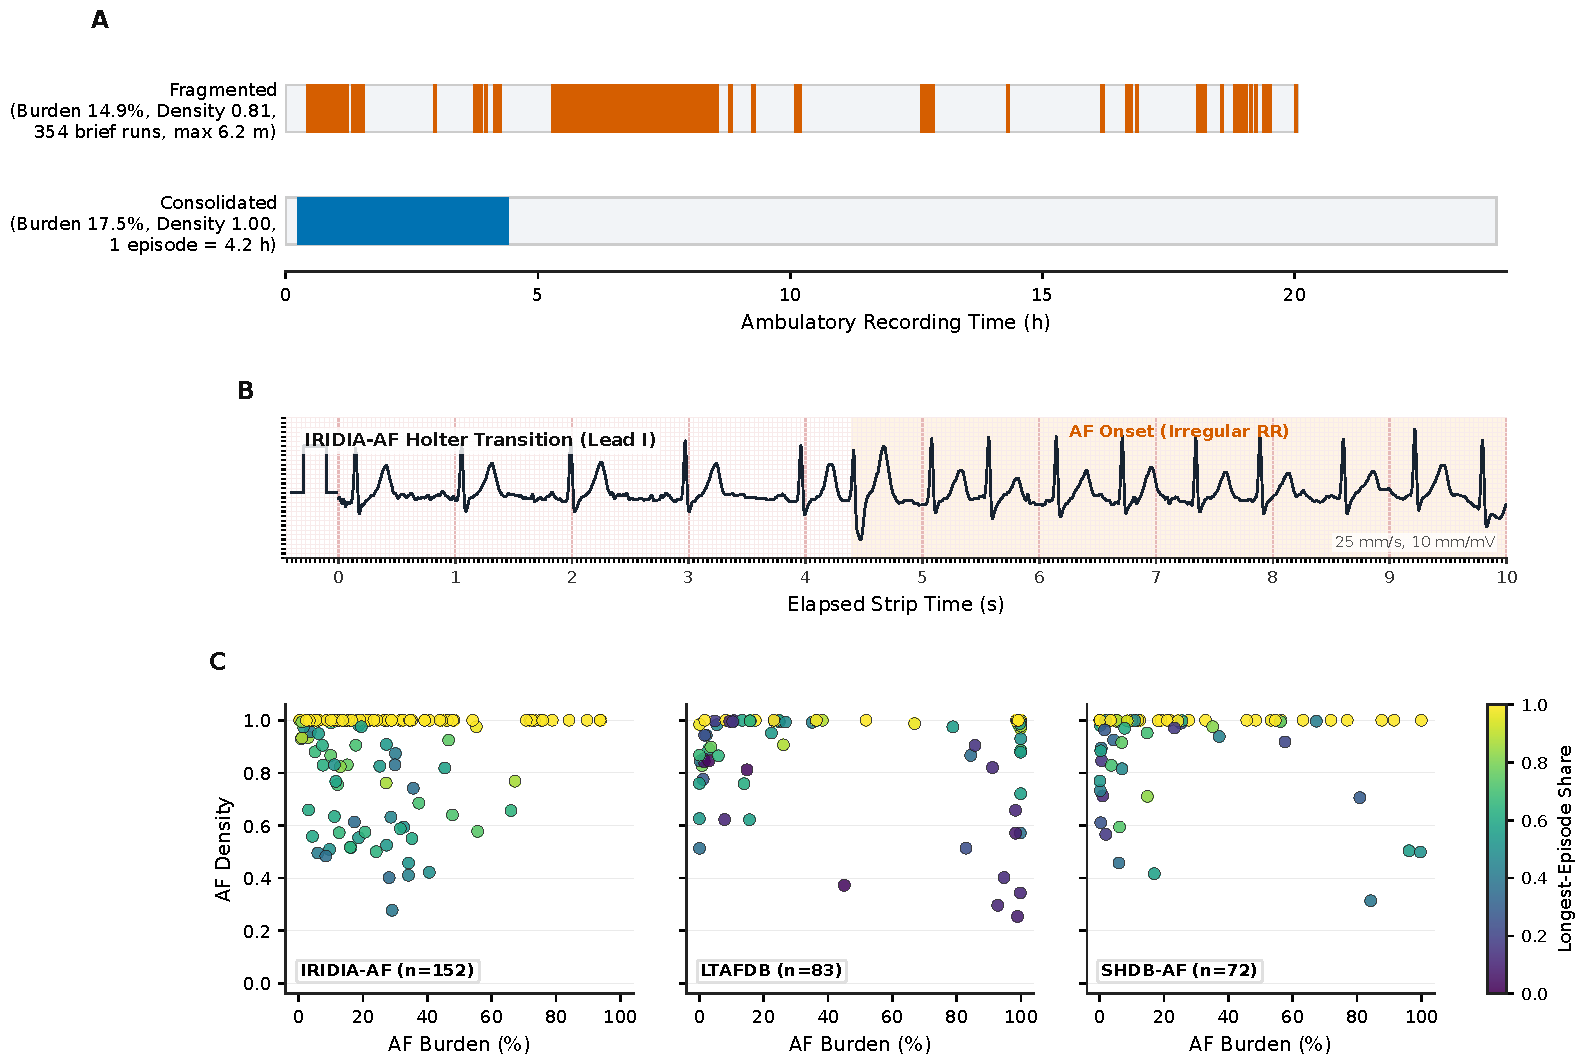
\includegraphics[width=0.95\textwidth]{figures_hrs/Fig01_temporal_phenotypes_and_ecg.pdf}
    \caption{Divergent temporal AF phenotypes at matched cumulative burden. (A) Paired 24-hour episode timelines illustrating fragmented brief-run AF (14.9\% burden, 354 brief runs, density 0.81) versus consolidated prolonged AF (17.5\% burden, single 4.2-hour episode, density 1.00). (B) Authentic 10-second Lead I ambulatory strip from IRIDIA-AF (25 mm/s, 10 mm/mV) capturing the abrupt transition into irregular AF. (C) Joint burden--density distribution across IRIDIA-AF ($n=152$), LTAFDB ($n=83$), and SHDB-AF ($n=72$) colored by longest-episode share.}
    \label{fig:temporal_phenotypes}
\end{figure*}

\begin{figure*}[t]
    \centering
    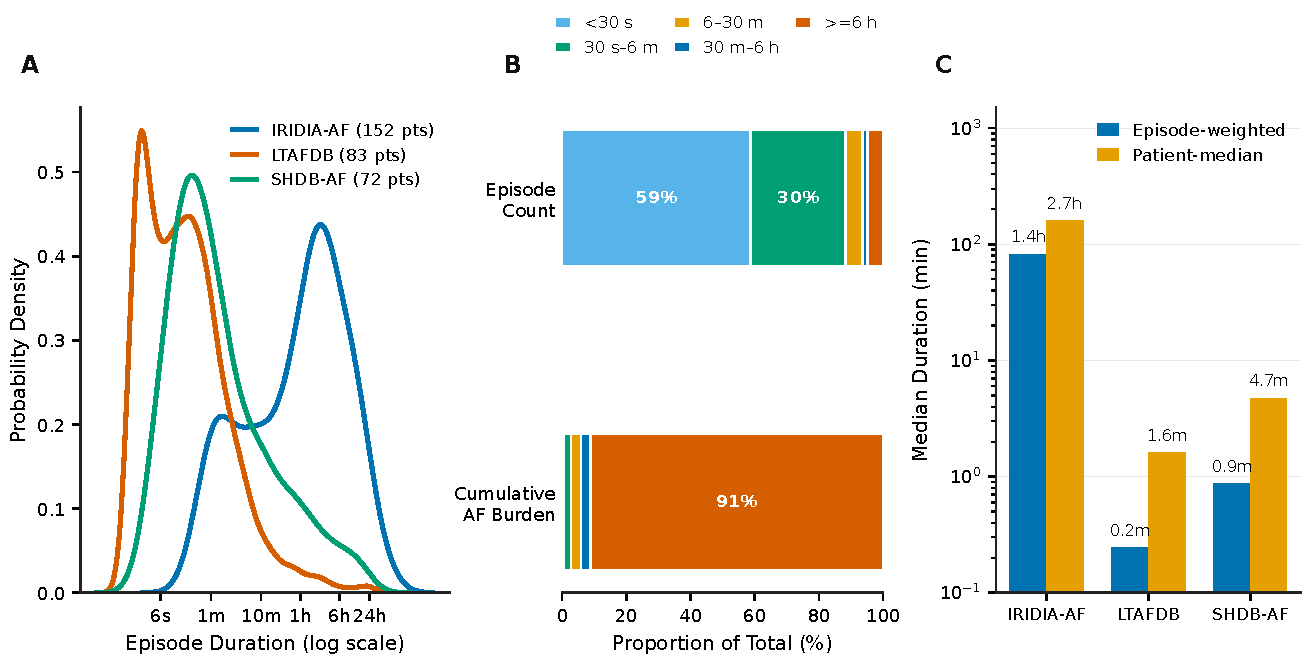
\includegraphics[width=0.95\textwidth]{figures_hrs/Fig02_cohort_duration_architecture.pdf}
    \caption{Episode-duration architecture across 349 ambulatory recordings (10,982 hours). (A) Log-scale episode duration density by cohort. (B) Contrasting share of episode count (59\% $<30$ s) versus cumulative AF burden (91\% $\ge 1$ h). (C) Divergence between episode-weighted and patient-averaged median durations.}
    \label{fig:duration_architecture}
\end{figure*}

\begin{figure*}[t]
    \centering
    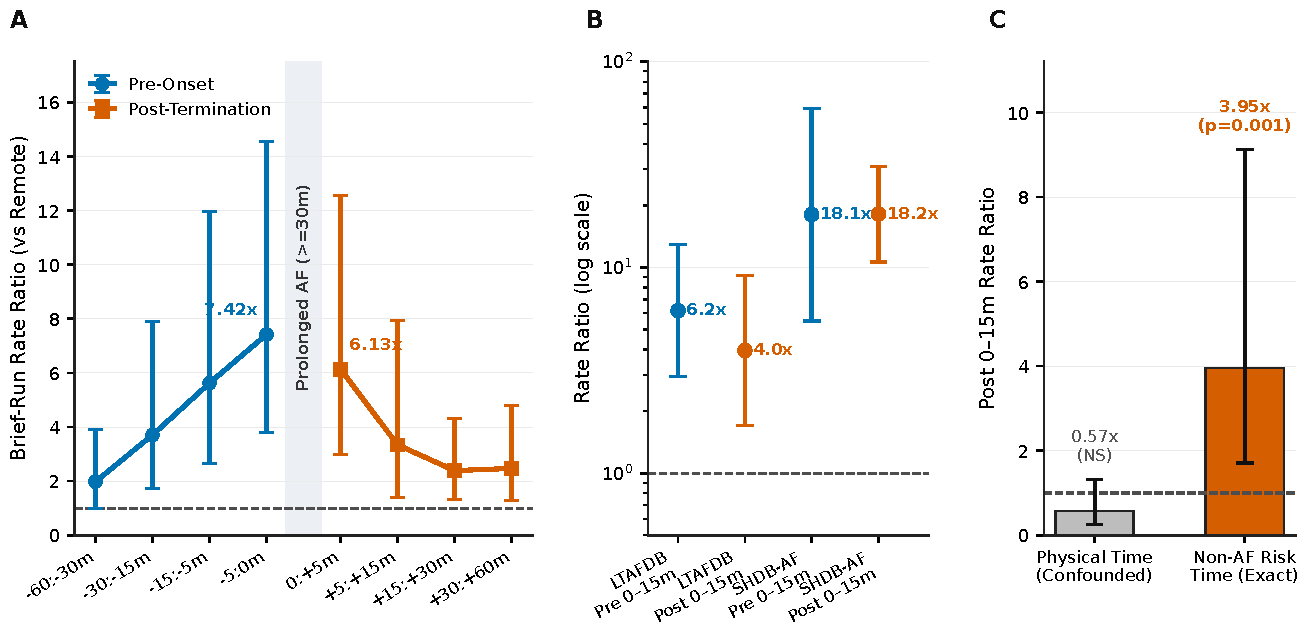
\includegraphics[width=0.95\textwidth]{figures_hrs/Fig03_neighbourhood_rate_surges.pdf}
    \caption{Temporal clustering of brief AF runs ($<30$ s) surrounding prolonged AF episodes ($\ge 30$ min). (A) Pooled risk-time rate ratios (95\% CI) showing pre-onset escalation (7.42-fold at 0--5 min) and immediate post-termination surge (6.13-fold at 0--5 min) relative to remote baseline. (B) Cohort stratification (0--15 min windows). (C) Artifactual attenuation (0.57-fold) when using physical time rather than non-AF risk time in LTAFDB.}
    \label{fig:neighbourhood_surges}
\end{figure*}

\begin{figure*}[t]
    \centering
    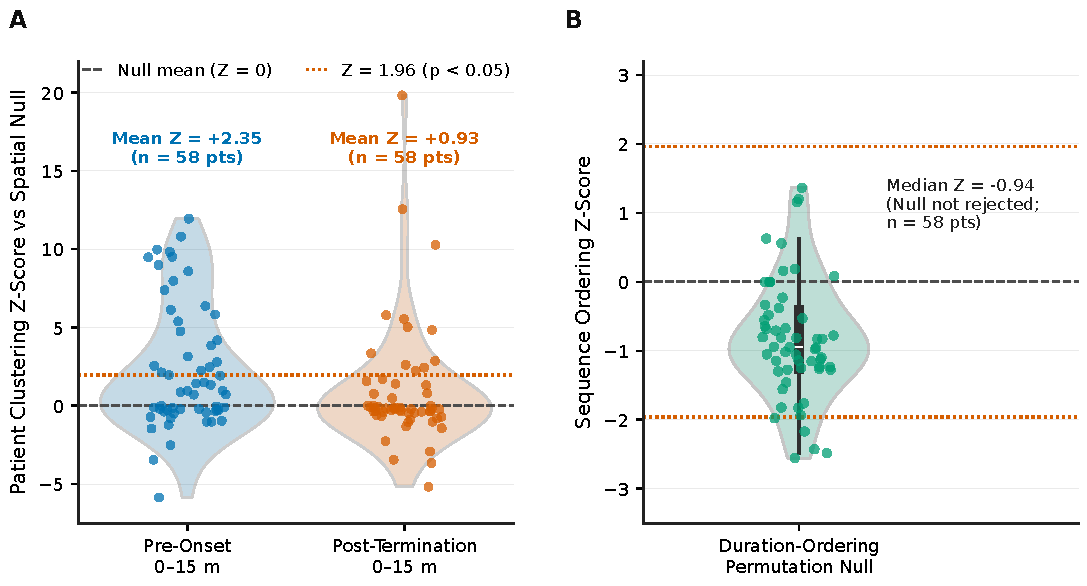
\includegraphics[width=0.95\textwidth]{figures_hrs/Fig04_conditional_null_validation.pdf}
    \caption{Conditional randomization validation across 58 eligible patients. (A) Patient-level clustering Z-scores relative to spatially shuffled brief runs (Null A). (B) Episode-duration sequence permutation test (Null B), confirming duration ordering does not exceed gap-duration marginals.}
    \label{fig:conditional_nulls}
\end{figure*}

\begin{figure*}[t]
    \centering
    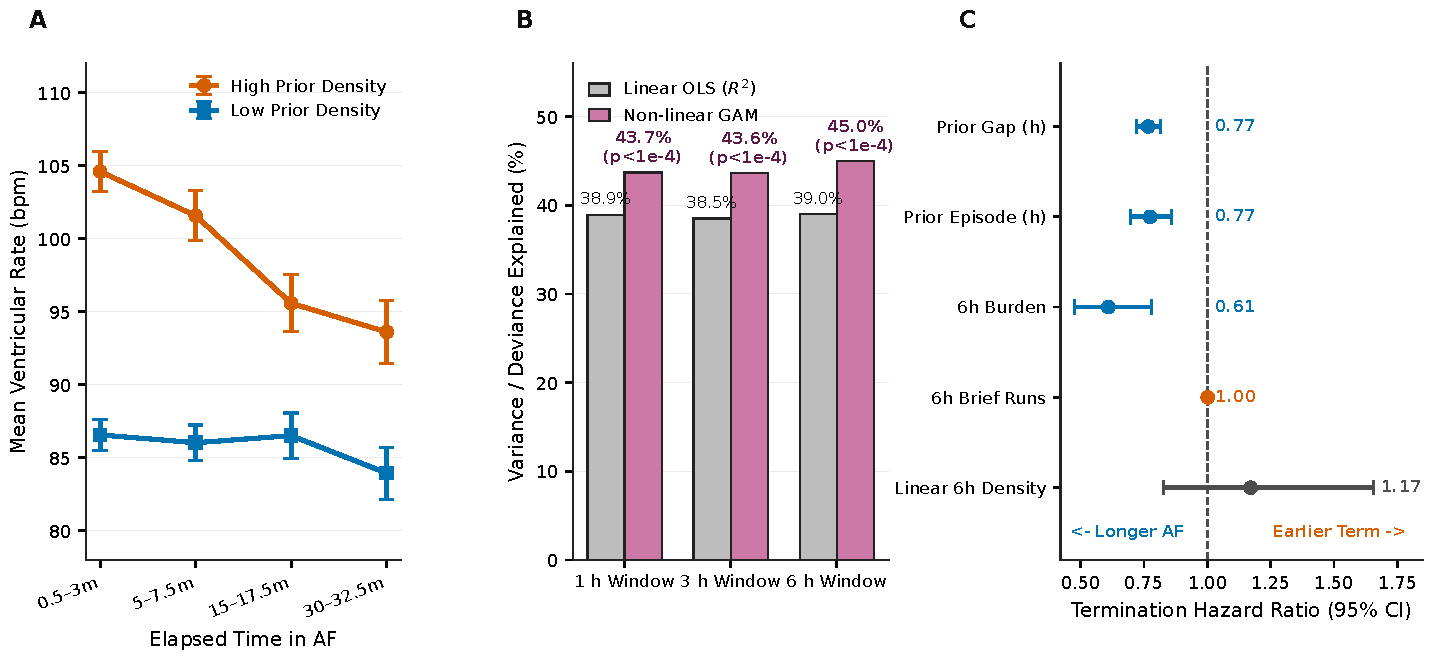
\includegraphics[width=0.95\textwidth]{figures_hrs/Fig05_acute_physiology_and_persistence.pdf}
    \caption{Electrophysiological evolution and subsequent episode persistence (E02). (A) Fixed elapsed-time ventricular rate stratified by high versus low preceding 6-hour AF density. (B) Non-linear generalized additive model (GAM) deviance explained versus linear regression for subsequent episode duration. (C) Cox proportional hazards termination ratios ($n=6,683$ episodes, 244 patients).}
    \label{fig:ep_persistence}
\end{figure*}

\begin{figure*}[t]
    \centering
    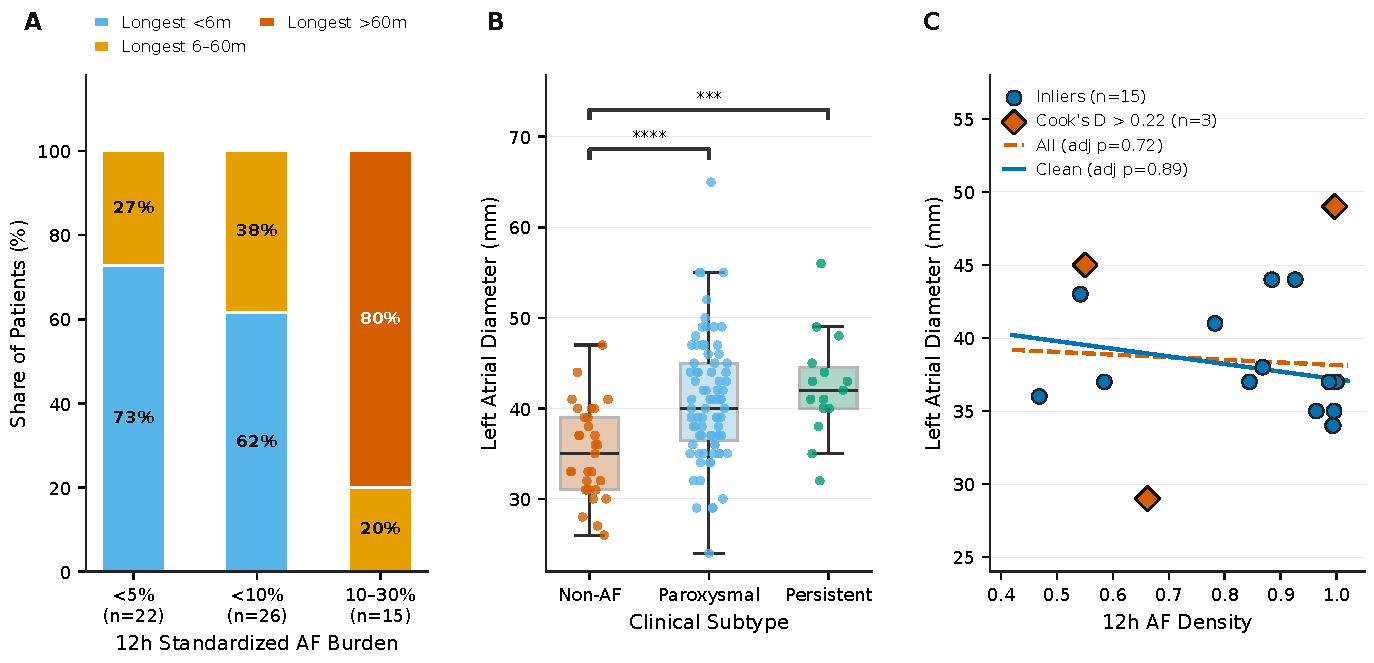
\includegraphics[width=0.95\textwidth]{figures_hrs/Fig06_shdb_clinical_substrate.pdf}
    \caption{Low-burden phenotype divergence and echocardiographic left atrial substrate in SHDB-AF (E03). (A) Longest-episode dominance across standardized 12-hour burden strata. (B) Left atrial diameter (LAD) across clinical subtypes. (C) Non-significant association between LAD and 12-hour AF density in contemporaneous paroxysmal AF ($\le 90$ days, $n=18$), highlighting 3 high-leverage patients (Cook's $D > 0.22$).}
    \label{fig:shdb_substrate}
\end{figure*}

\begin{figure*}[t]
    \centering
    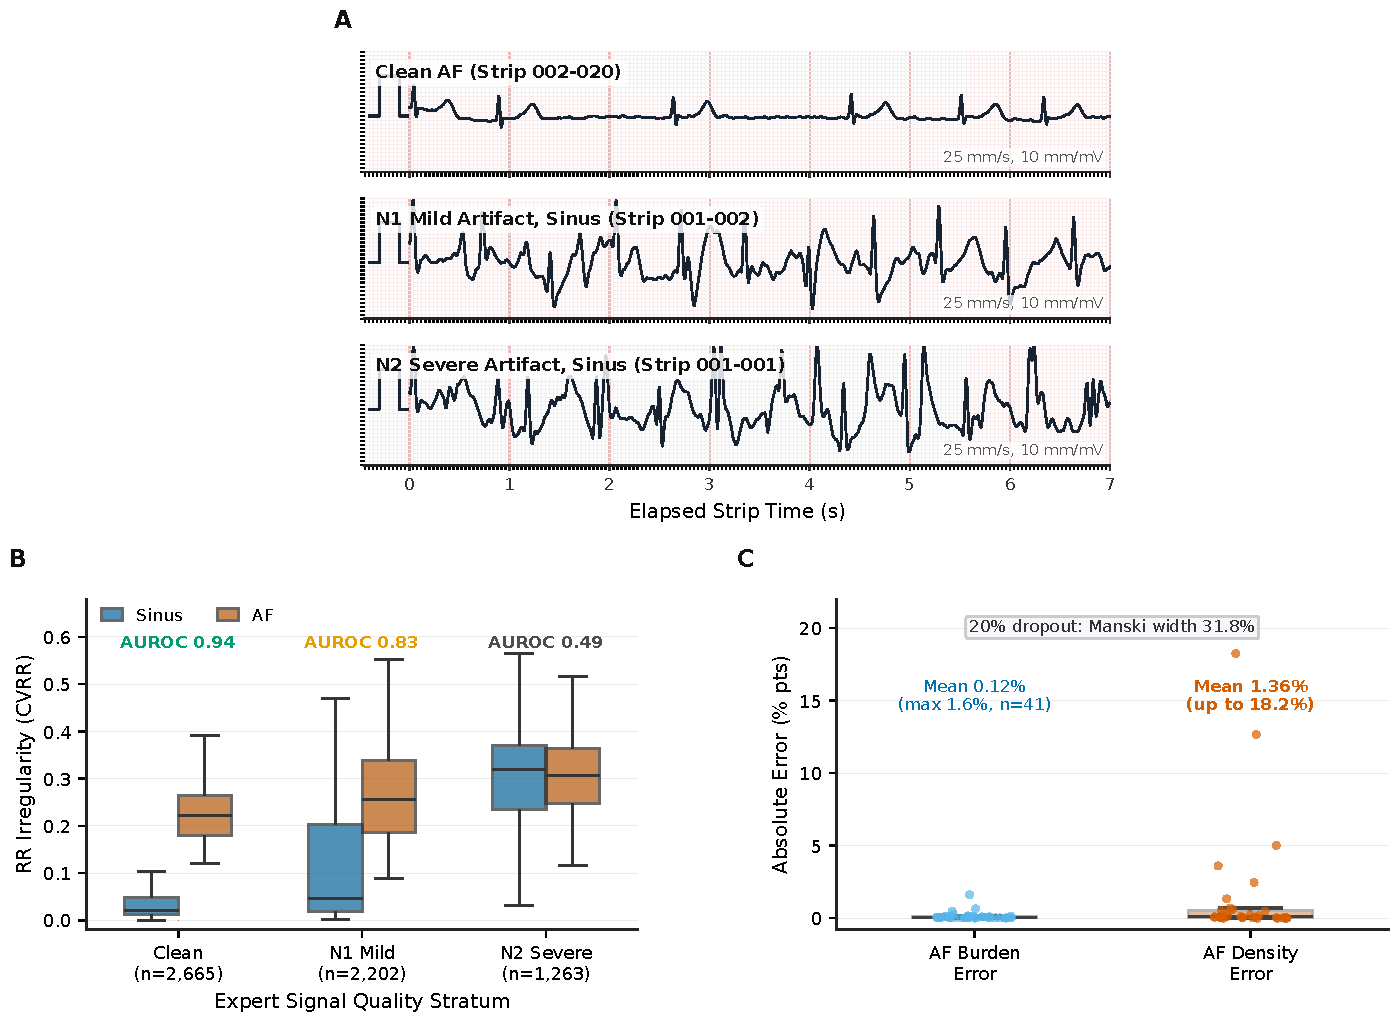
\includegraphics[width=0.95\textwidth]{figures_hrs/Fig07_noise_observability_and_ecg.pdf}
    \caption{Impact of authentic ambulatory ECG artifact on HRV and AF density (E04). (A) Calibrated 25 mm/s, 10 mm/mV Holter strips across Clean AF, mild artifact (N1), and severe artifact (N2). (B) Collapse of RR irregularity (CVRR) discrimination between sinus rhythm and AF from Clean (AUROC 0.94) to N2 noise (0.49). (C) Cumulative burden resilience ($<0.2\%$ error) versus density distortion (up to 18.2\% error) upon omitting brief runs.}
    \label{fig:noise_observability}
\end{figure*}

\begin{figure*}[t]
    \centering
    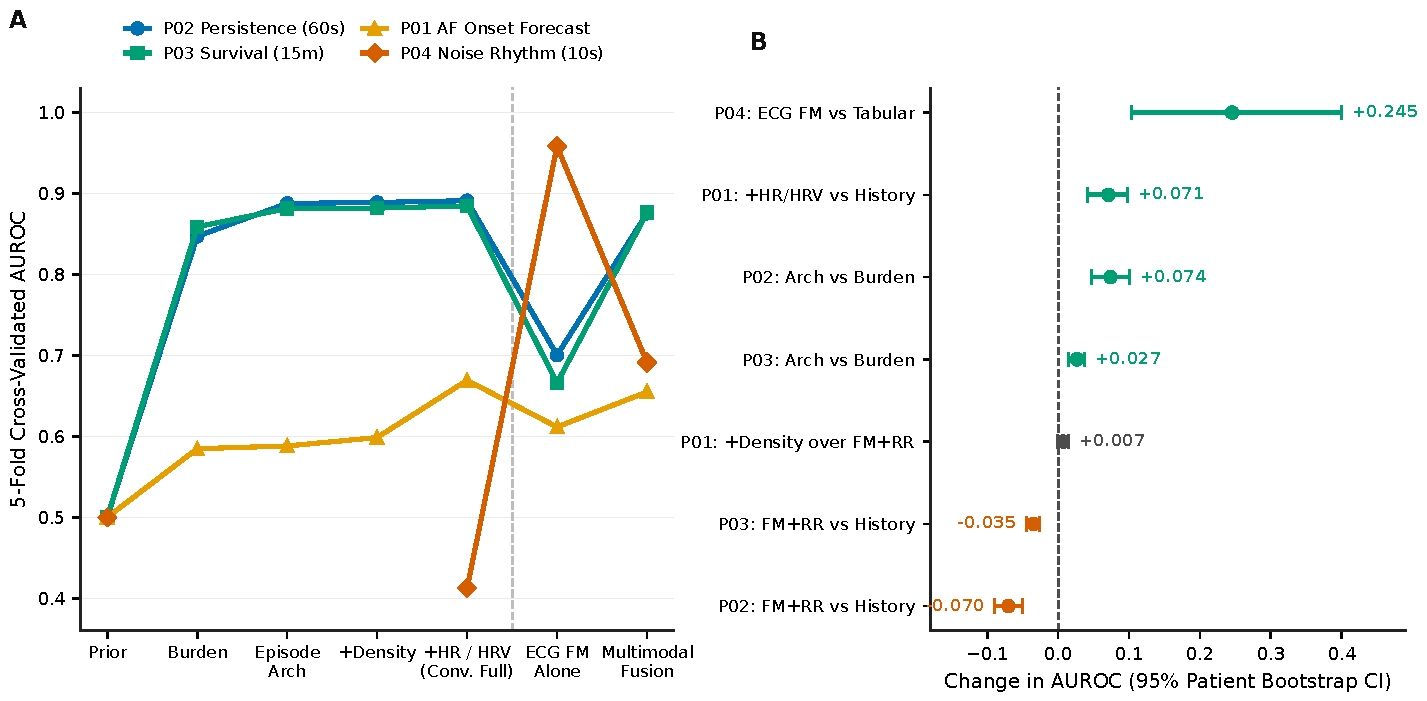
\includegraphics[width=0.95\textwidth]{figures_hrs/Fig08_ablation_and_bootstrap_contrasts.pdf}
    \caption{Incremental value of longitudinal rhythm history versus instantaneous ECG representations (V7-P). (A) Cross-validated AUROC progression across clinical information tiers for P01--P04. (B) Patient-clustered bootstrap contrasts (95\% CI) separating longitudinal prognostic gain from instantaneous noisy-strip classification.}
    \label{fig:ablation_contrasts}
\end{figure*}

\begin{figure*}[t]
    \centering
    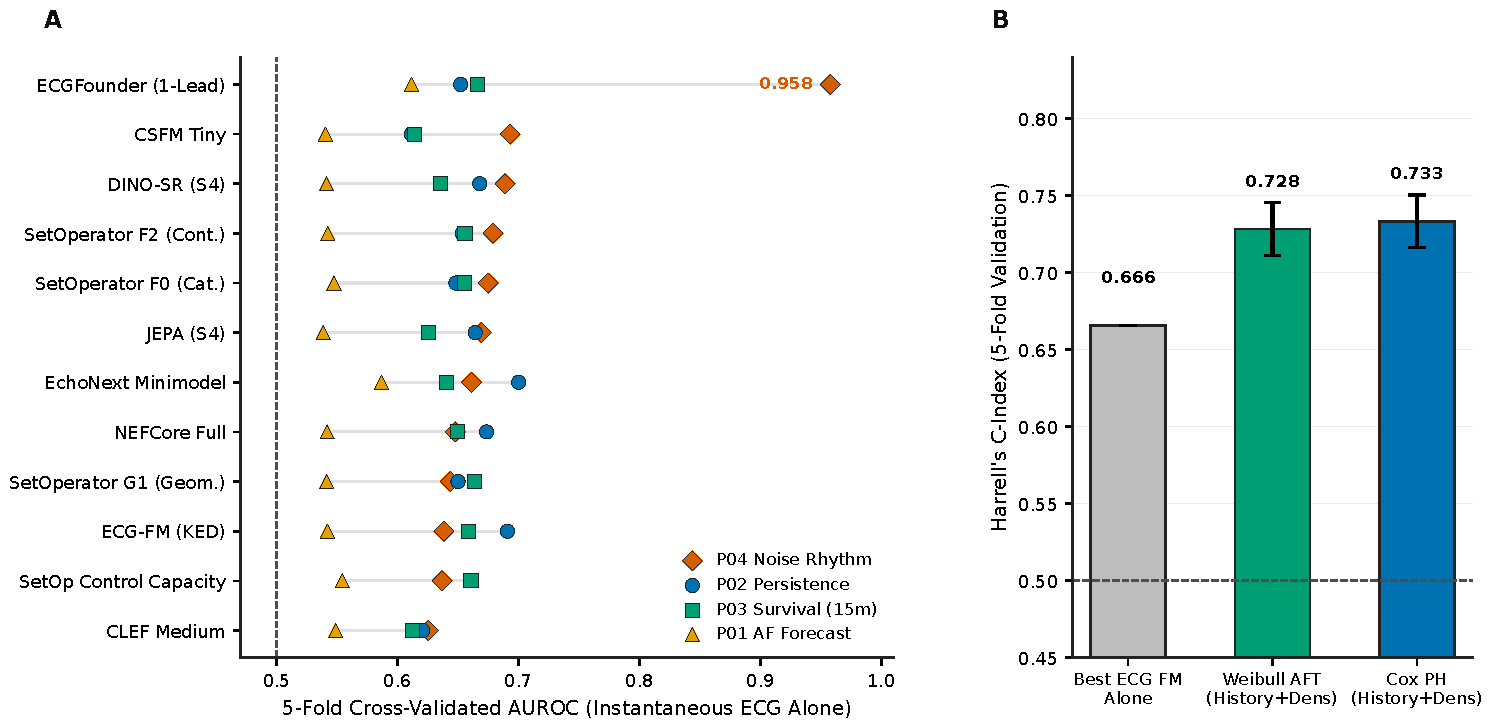
\includegraphics[width=0.95\textwidth]{figures_hrs/Fig09_foundation_models_and_survival.pdf}
    \caption{Evaluation of 12 pretrained ECG foundation models and continuous SetOperators. (A) Cross-validated AUROC across instantaneous rhythm detection (P04) versus longitudinal episode prognosis (P01--P03). (B) 5-fold Harrell's C-index for dynamic episode termination survival (P03).}
    \label{fig:fm_and_survival}
\end{figure*}

\begin{figure*}[t]
    \centering
    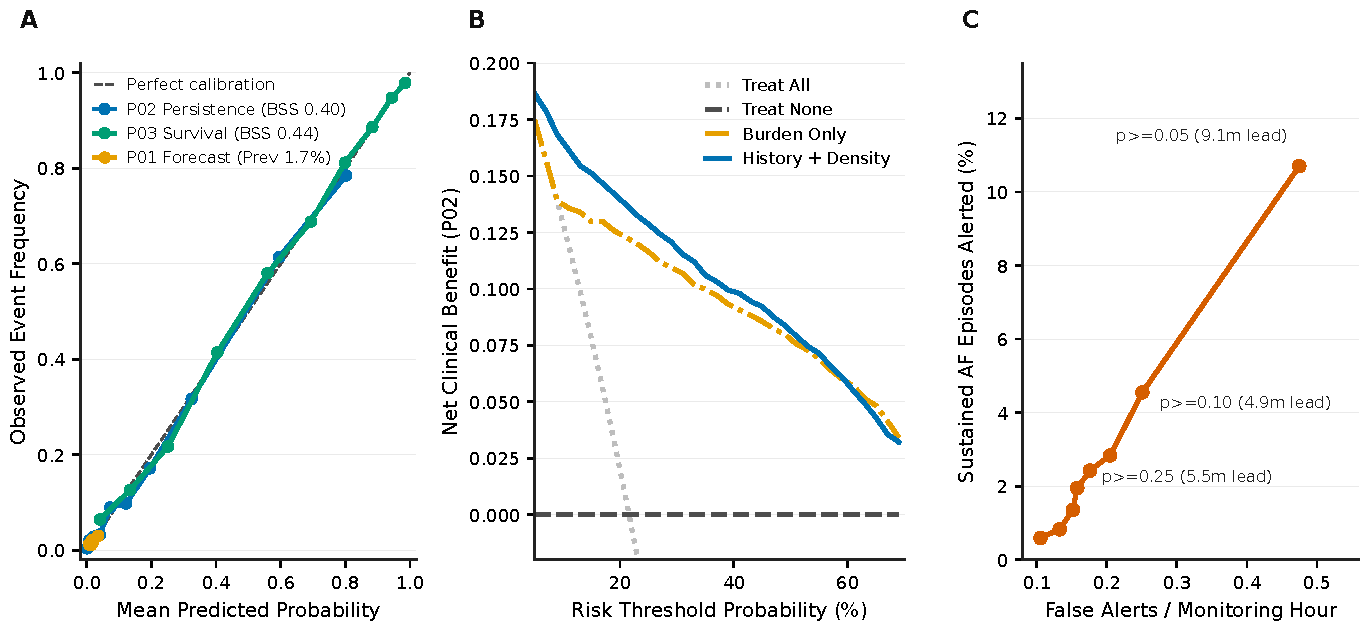
\includegraphics[width=0.95\textwidth]{figures_hrs/Fig10_calibration_dca_and_alerts.pdf}
    \caption{Clinical calibration, decision curve net benefit, and continuous warning trade-off. (A) Out-of-fold calibration curves across 3.05 million predictions. (B) Decision curve analysis (dcurves) showing Net Benefit for 60-second episode persistence triage (P02). (C) Alert sensitivity versus false-alert burden for imminent sustained AF forecasting (P01).}
    \label{fig:calibration_dca}
\end{figure*}
